% Figure 1 — the CertGate pipeline (schematic; no data content).
% Standalone TikZ; compiled by paper/make_submission.py into figs/pipeline.pdf.
% Journal artwork rules honoured: sans-serif lettering; information never
% carried by colour alone (fills are paired with border styles: solid =
% data pool, thick = fitted object, double = certified output, dashed =
% decline/abstain path).
\documentclass[tikz,border=10pt]{standalone}
\usetikzlibrary{arrows.meta}
\renewcommand{\familydefault}{\sfdefault}
\begin{document}
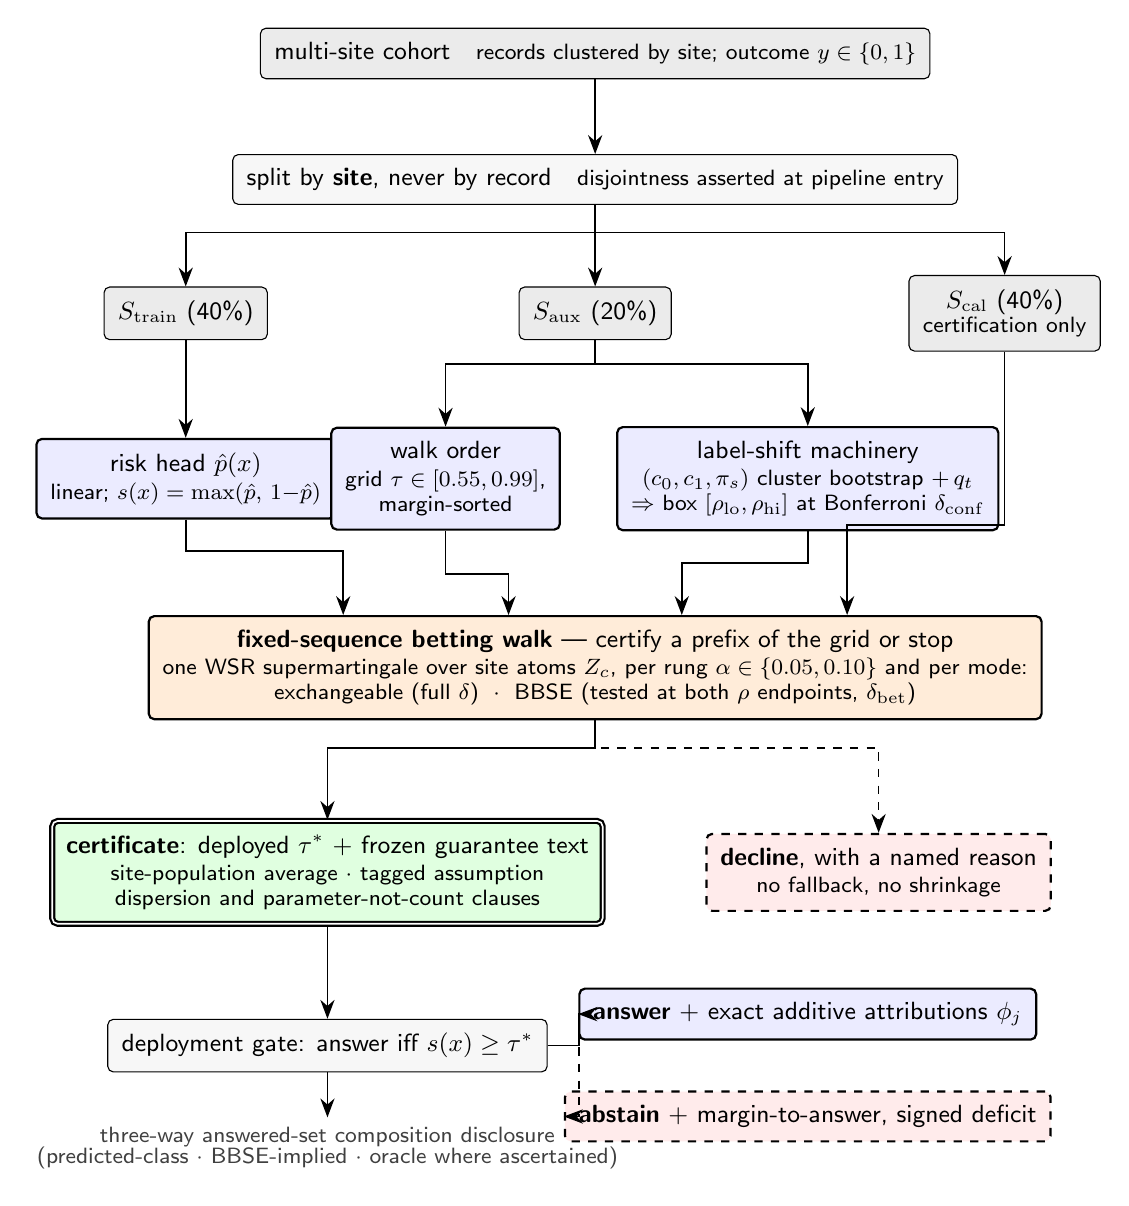
\begin{tikzpicture}[
  font=\small,
  box/.style={draw, rounded corners=2pt, align=center, inner sep=5pt},
  pool/.style={box, fill=black!8},
  stage/.style={box, thick, fill=blue!8},
  cert/.style={box, double, thick, fill=green!12},
  dec/.style={box, dashed, thick, fill=red!8},
  note/.style={font=\footnotesize, text=black!75, align=center},
  arr/.style={-{Stealth[length=2.4mm]}, semithick},
  darr/.style={arr, dashed}
]

% row 1-2: cohort and split
\node[pool] (cohort) at (7,0)
  {multi-site cohort\quad {\footnotesize records clustered by site; outcome $y\in\{0,1\}$}};
\node[box, fill=black!3] (split) at (7,-1.6)
  {split by \textbf{site}, never by record\quad {\footnotesize disjointness asserted at pipeline entry}};
\draw[arr] (cohort) -- (split);

% row 3: the three pools
\node[pool] (train) at (1.8,-3.3)  {$S_{\mathrm{train}}$ (40\%)};
\node[pool] (aux)   at (7,-3.3)    {$S_{\mathrm{aux}}$ (20\%)};
\node[pool] (cal)   at (12.2,-3.3) {$S_{\mathrm{cal}}$ (40\%)\\[-2pt] \footnotesize certification only};
\draw[arr] (split.south) -- ++(0,-0.35) -| (train.north);
\draw[arr] (split.south) -- (aux.north);
\draw[arr] (split.south) -- ++(0,-0.35) -| (cal.north);

% row 4: fitted objects
\node[stage] (head) at (1.8,-5.4)
  {risk head $\hat p(x)$\\[-1pt] \footnotesize linear; $s(x)=\max(\hat p,\,1{-}\hat p)$};
\node[stage] (order) at (5.1,-5.4)
  {walk order\\[-1pt] \footnotesize grid $\tau\in[0.55,0.99]$,\\[-2pt] \footnotesize margin-sorted};
\node[stage] (bbse) at (9.7,-5.4)
  {label-shift machinery\\[-1pt] \footnotesize $(c_0,c_1,\pi_s)$ cluster bootstrap $+\,q_t$\\[-2pt] \footnotesize $\Rightarrow$ box $[\rho_{\mathrm{lo}},\rho_{\mathrm{hi}}]$ at Bonferroni $\delta_{\mathrm{conf}}$};
\draw[arr] (train) -- (head);
\draw[arr] (aux.south) -- ++(0,-0.3) -| (order.north);
\draw[arr] (aux.south) -- ++(0,-0.3) -| (bbse.north);

% row 5: the certification walk
\node[box, thick, fill=orange!15] (walk) at (7,-7.8)
  {\textbf{fixed-sequence betting walk} --- certify a prefix of the grid or stop\\[-1pt]
   \footnotesize one WSR supermartingale over site atoms $Z_c$, per rung $\alpha\in\{0.05,0.10\}$ and per mode:\\[-2pt]
   \footnotesize exchangeable (full $\delta$) $\;\cdot\;$ BBSE (tested at both $\rho$ endpoints, $\delta_{\mathrm{bet}}$)};
\draw[arr] (head.south)  -- ++(0,-0.4) -| ([xshift=-3.2cm]walk.north);
\draw[arr] (order.south) -- ++(0,-0.55) -| ([xshift=-1.1cm]walk.north);
\draw[arr] (bbse.south)  -- ++(0,-0.4) -| ([xshift=1.1cm]walk.north);
\draw[arr] (cal.south)   -- ++(0,-2.2) -| ([xshift=3.2cm]walk.north);

% row 6: certificate or decline
\node[cert] (certif) at (3.6,-10.4)
  {\textbf{certificate}: deployed $\tau^{*}$ $+$ frozen guarantee text\\[-1pt]
   \footnotesize site-population average $\cdot$ tagged assumption\\[-2pt]
   \footnotesize dispersion and parameter-not-count clauses};
\node[dec] (decline) at (10.6,-10.4)
  {\textbf{decline}, with a named reason\\[-1pt] \footnotesize no fallback, no shrinkage};
\draw[arr]  (walk.south) -- ++(0,-0.35) -| (certif.north);
\draw[darr] (walk.south) -- ++(0,-0.35) -| (decline.north);

% row 7: deployment
\node[box, fill=black!3] (gate) at (3.6,-12.6)
  {deployment gate: answer iff $s(x)\ge\tau^{*}$};
\node[stage] (ans) at (9.7,-12.2)
  {\textbf{answer} $+$ exact additive attributions $\phi_j$};
\node[dec] (abst) at (9.7,-13.5)
  {\textbf{abstain} $+$ margin-to-answer, signed deficit};
\node[note] (comp) at (3.6,-13.9)
  {three-way answered-set composition disclosure\\[-2pt] (predicted-class $\cdot$ BBSE-implied $\cdot$ oracle where ascertained)};
\draw[arr]  (certif) -- (gate);
\draw[arr]  (gate.east) -- ++(0.4,0) |- (ans.west);
\draw[darr] (gate.east) -- ++(0.4,0) |- (abst.west);
\draw[arr]  (gate) -- (comp);

\end{tikzpicture}
\end{document}
